\documentclass{article}
\usepackage{geometry}
\geometry{
    top = 0.75in,
    bottom = 0.75in,
    right = 0.75in,
    left = 0.75in,
}
\usepackage{amsmath}
\usepackage{graphicx}
\usepackage{parskip}

\author{Mani Setayesh, Leon Cai}
\title{CSC258 - Breakout Project Report}
\begin{document}
\maketitle
\section*{Memory Layout}
Things that need to be laid out:\begin{itemize}
\item A ball - it should have $(x,y)$ values, in addition to the ``direction" of the ball. The direction of the ball follows an encoding - e.g. if a value of 1 is stored, then direction is left, etc.
\item A paddle - it only needs $(x,y)$ values (frankly not even the $y$ value since the paddle only moves horizontally).
\item Colours - just an array of the colours used in the display. Multiple colours (one for each row), and 3 monochrome colours (black,gray,white) stored at the end- used for the ball, the paddle, the walls, and empty space.
\end{itemize}
Memory layout at the beginning:
\begin{figure}[ht!]
    \centering
    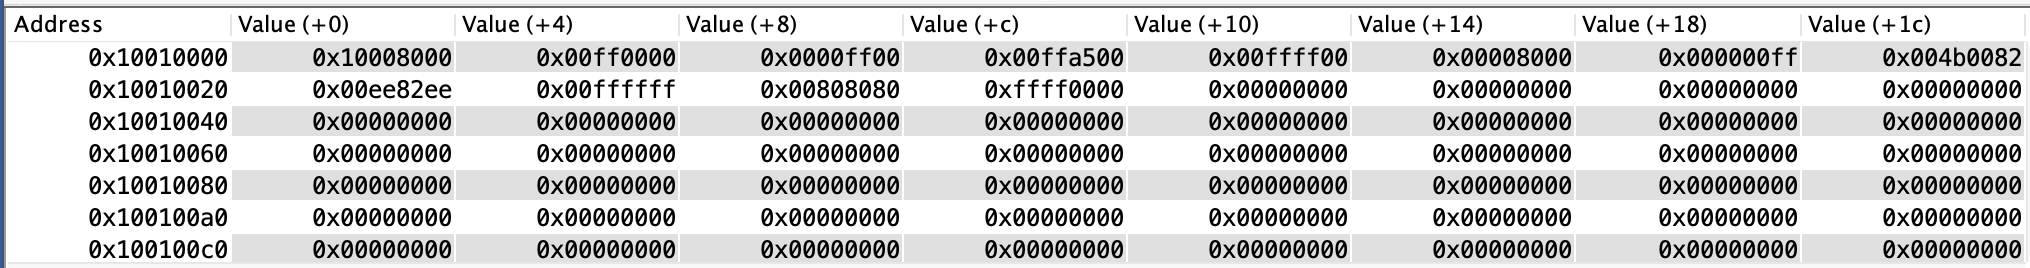
\includegraphics[width=0.5\textwidth]{memory_layout.png}
    \caption{Initial memory}
\end{figure}\\
The values in the memory include the keyboard display address (ADDR\_DSPL) - given already in the file. Then the array of 10  colours, then spaces left for the $x,y$ values of the ball and paddle. It is hard to get the memory's layout for the walls and bricks in one picture, as what we will have is: \begin{figure}[ht!]
    \centering
    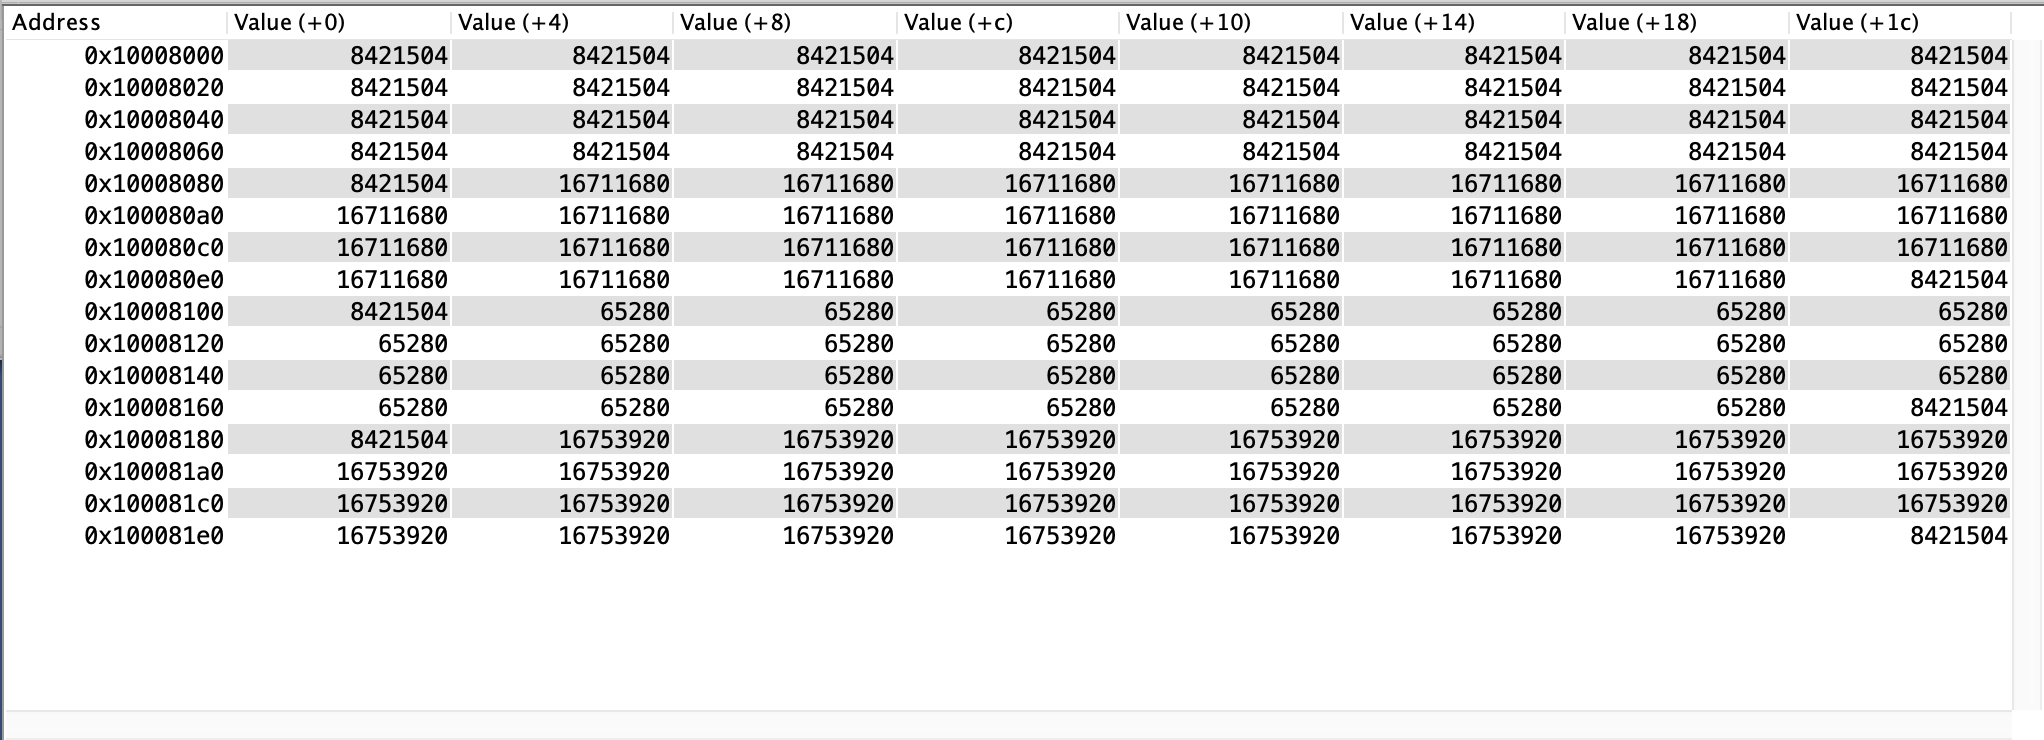
\includegraphics[width=0.5\textwidth]{colours.png}
    \caption{Coloured memory}
\end{figure}\\ Notice that the repeated numbers each indicate a row from the top - the top row is coloured gray, done by storing ``gray" values into 32 word spaces (each representing a pixel). Then a row of red, then green, then etc.
Here is a screen-shot of the static scene (at Statthe start of the game):\begin{figure}[ht!]
    \centering
    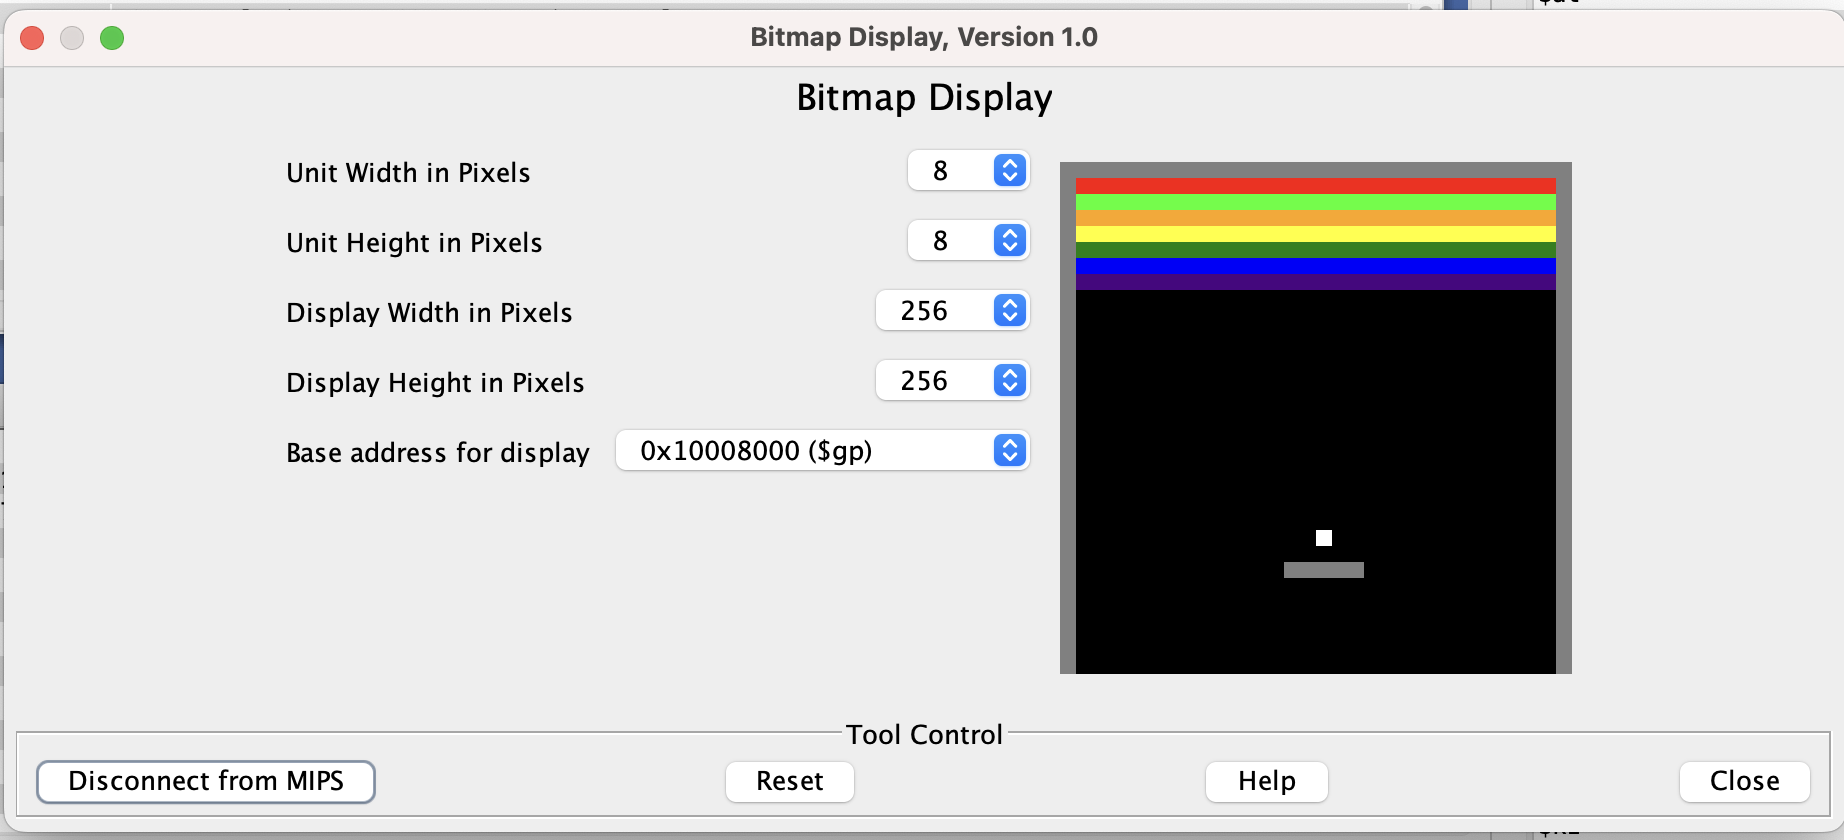
\includegraphics[width=0.3\textwidth]{static_scene.png}
    \caption{Static scene}
\end{figure}\newpage
\section*{Dealing with collisions}
The main aspect with dealing with a collision is changing the already stored ``direction" value (gotten from address: BALL + 8)  to a new direction that the ball should go in. Using classic breakout as reference, the ball mainly moves in diagonals. We associate each diagonal with a number from 1-4: Up-right = 1, Up-left = 2, Down-left = 3, Down-right = 4 (cntr clkwise from top-right). The general idea is for the ball's direction to rotate 90 degrees when it hits anything - though the direction of the rotation should be intuitive:
\begin{itemize}
\item Ball hits the paddle - in this case, the ball should only change whether its going up/down, not left/right. For example, if it hits the paddle with dir = 3, then the new dir would be 2. If it hits the paddle with dir = 4, then the new dir would be 1.
\item Ball hits a wall: Differentiating top walls from side walls, we have the direction that should change and that should not change. For the side wall collision, the ball should keep its vertical direction  - but it should change its horizontal direction (if going left, hit the left wall, then go right). For the top wall, its the other way around - keep the horizontal direction, but instead of going up the ball will go down. If it hits a corner, then the new direction is the opposite of the old direction (going up-right, hit corner, go down-left).
\item Ball hits a brick - the same idea as hitting the top wall.
\end{itemize}
Here is a visual diagram for how it the bouncing directions would work:\begin{figure}[ht!]
    \centering
    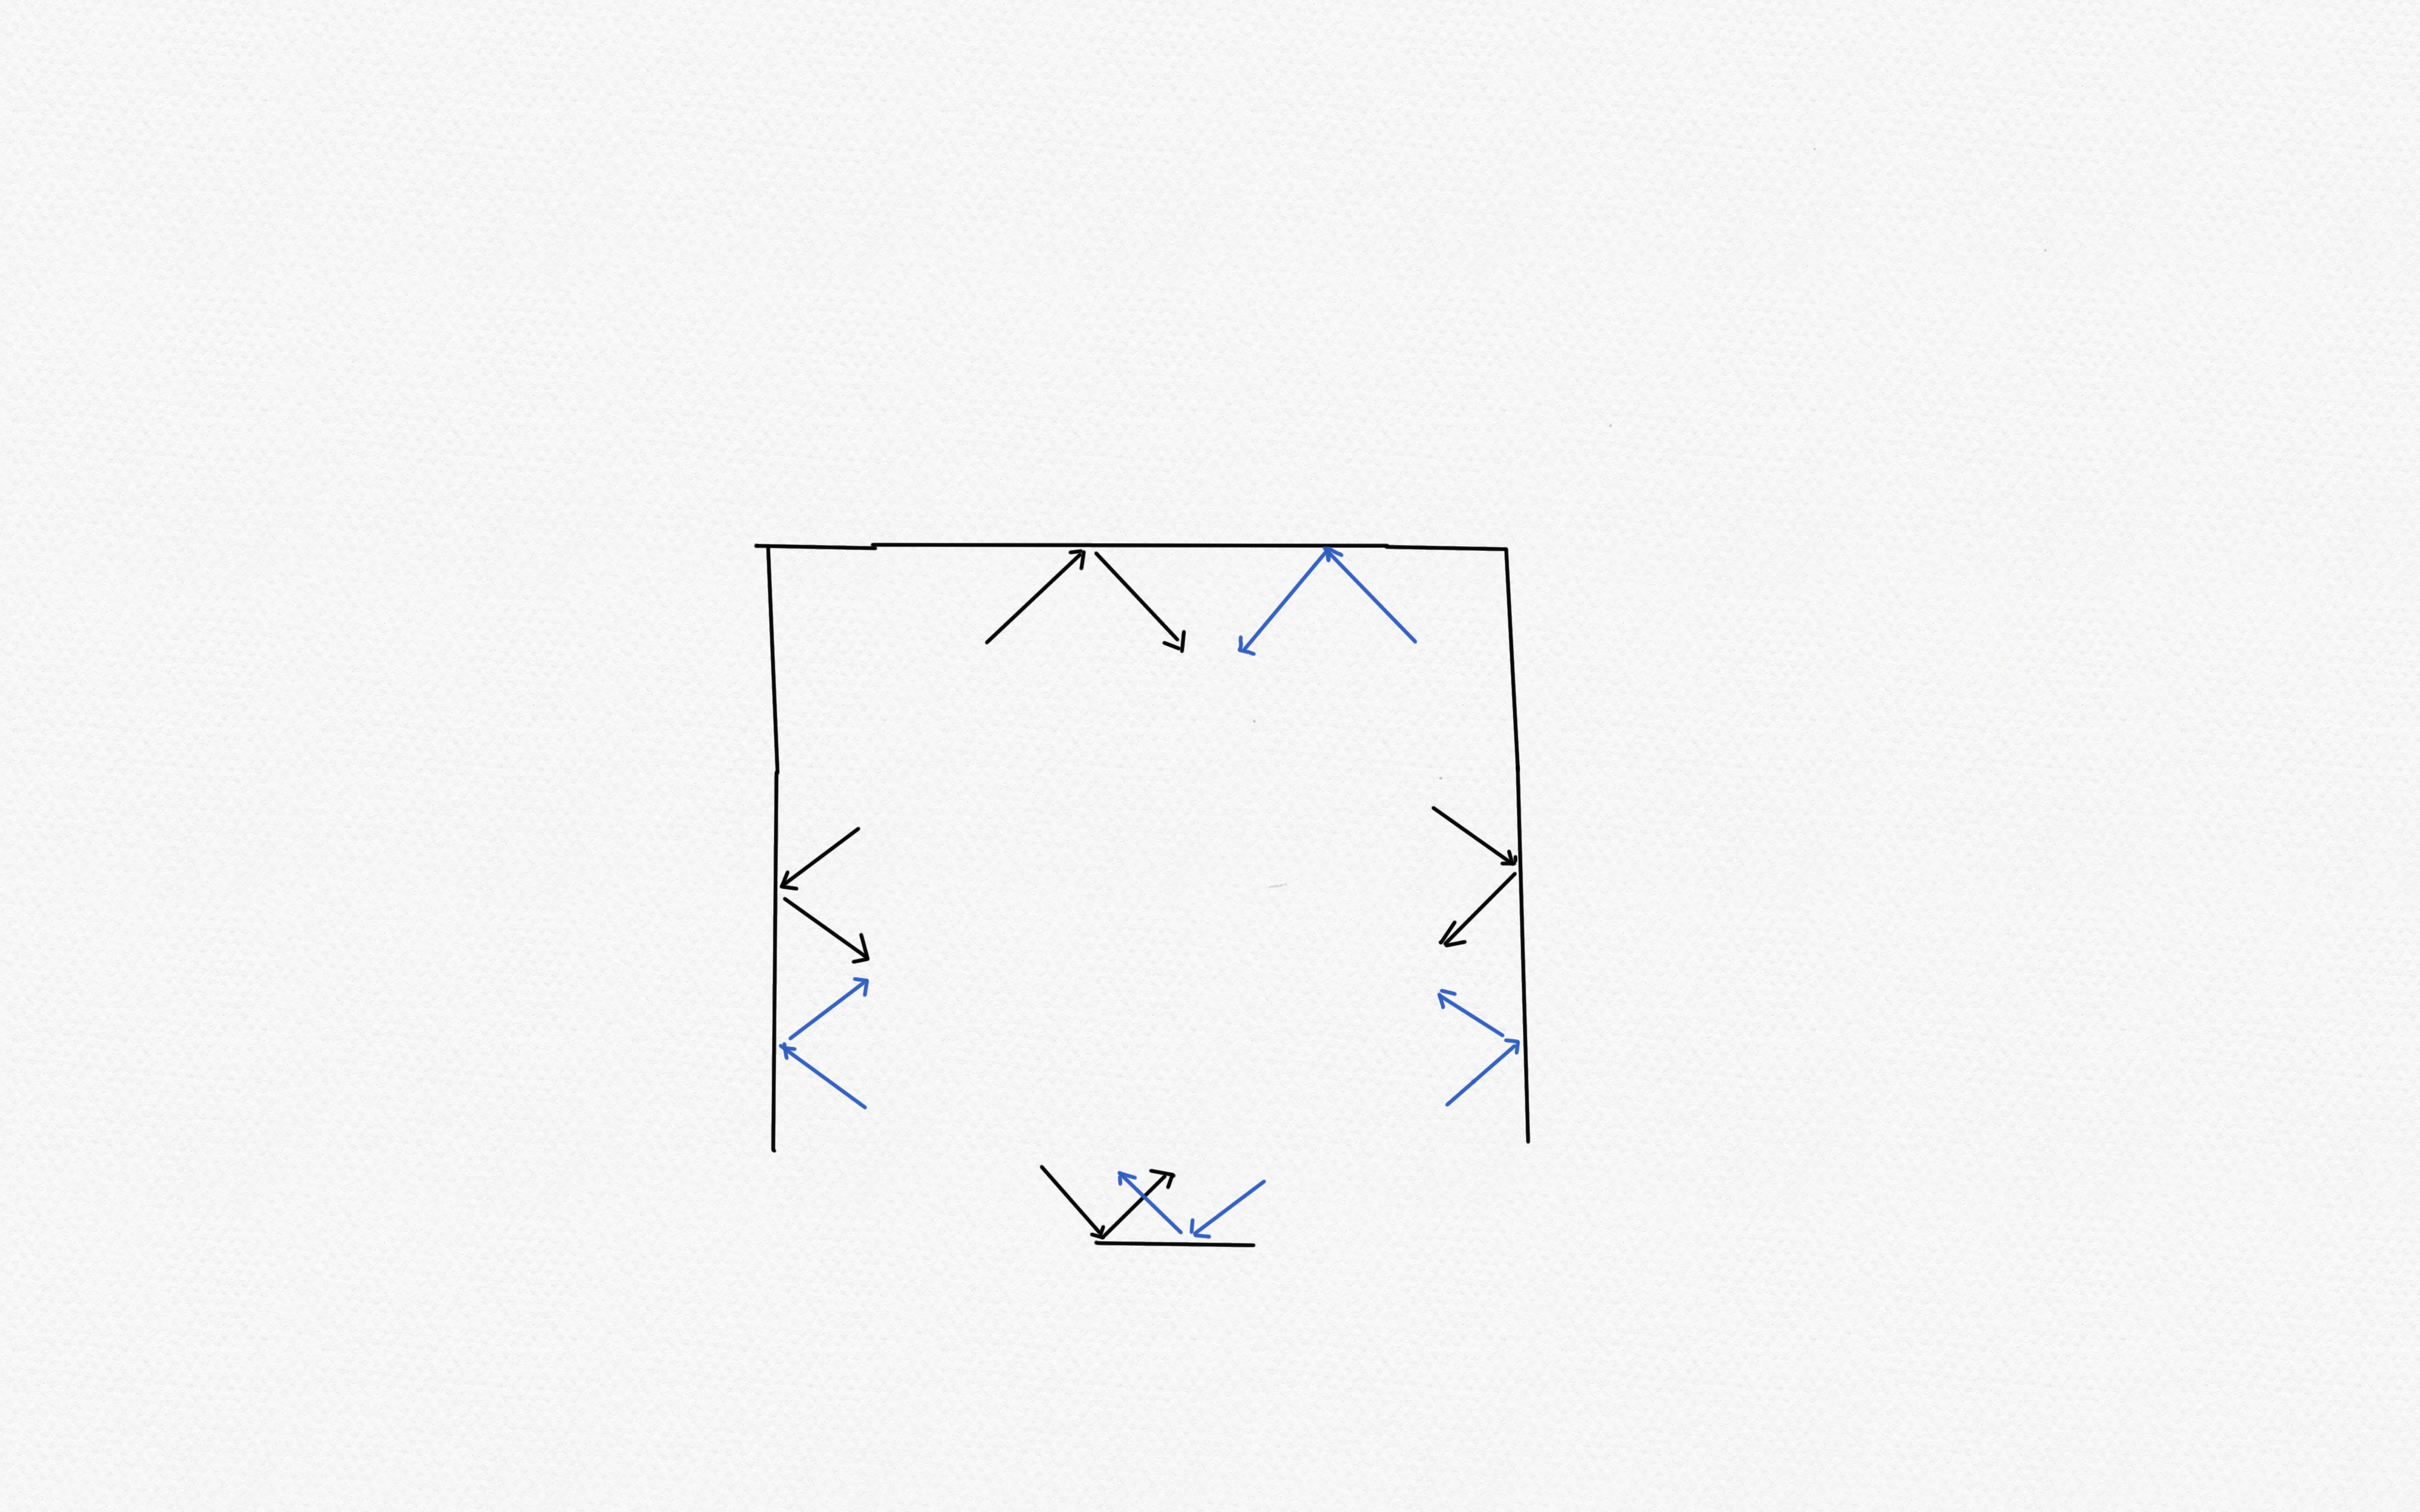
\includegraphics[width=0.7\textwidth]{collisions.png}
    \caption{Collisions, relative to wall/paddle}
\end{figure}\\ 

\end{document}